\documentclass[conference,10pt,letterpaper]{IEEEtran}
\usepackage[T1]{fontenc}
\usepackage{amsmath,booktabs,graphicx,url,tikz,float,multirow}
\usetikzlibrary{arrows.meta,positioning}
\definecolor{csiBlue}{RGB}{34,105,158}
\definecolor{radarOrange}{RGB}{198,93,34}
\definecolor{fusionRed}{RGB}{156,40,67}
\renewcommand{\topfraction}{.95}
\renewcommand{\dbltopfraction}{.95}
\renewcommand{\textfraction}{.04}
\renewcommand{\floatpagefraction}{.85}
\renewcommand{\dblfloatpagefraction}{.85}
\setcounter{topnumber}{4}
\setcounter{dbltopnumber}{4}
\graphicspath{{icc_assets/}}
\title{Explainable and private LLM-based Occupancy Detection Model Framework with Multi-Modal Wireless Sensing:\\WiFi CSI and FMCW Radar}
\author{\IEEEauthorblockN{Gad Gad\IEEEauthorrefmark{1}, Mostafa Fouda\IEEEauthorrefmark{2}, Zubair Md Fadlullah\IEEEauthorrefmark{1}}
\IEEEauthorblockA{\IEEEauthorrefmark{1}Department of Computer Science, Western University, London, ON, Canada\\
\IEEEauthorrefmark{2}Department of Electrical and Computer Engineering, Idaho State University, Pocatello, ID, USA}}
\begin{document}
\maketitle
\begin{abstract}

Human occupancy detection using wireless sensing provides private continuous monitoring, but signal instability and distribution shift challenge model performance. Machine-learning predictions also offer limited explanations. We combine WiFi channel-state information (CSI) and frequency-modulated continuous-wave (FMCW) radar to predict room occupancy. Physical descriptors and trained-model probabilities are supplied to large language models (LLMs) for a prediction and textual rationale. We evaluate CSI, radar, early feature fusion, and late probability fusion on five-second windows and minute averages; validation data select models and thresholds before multilink test evaluation. The five-second models combine the physical descriptors with training-fitted PCA coordinates. Among the validation-selected models, CSI GBM achieves .929/.939 validation/test minute accuracy, radar GBM .741/.922, early-fusion GBM .929/.942, and late-fusion GBM .933/.986. GPT-4o mini scores $68.8\pm0.4$\% validation and $59.7\pm1.2$\% test accuracy, while GPT-5.4 scores $96.0\pm0.0$\% and $95.7\pm0.3$\%, respectively. Neither LLM exceeds the late-fusion GBM on test, and their rationales can repeat the supplied model predictions.

\end{abstract}
\begin{IEEEkeywords}
occupancy sensing, WiFi CSI, FMCW radar, domain shift, calibration
\end{IEEEkeywords}

\section{Introduction}
Room occupancy is a basic input for lighting, heating, and ventilation control, security, and in-home care. Camera-based occupancy detection raises privacy concerns, and wearable or infrared alternatives require cooperation or line of sight. Radio-frequency sensing offers a passive alternative: WiFi channel-state information (CSI) from commodity transceivers reflects multipath changes caused by a human body, and millimeter-wave frequency-modulated continuous-wave (FMCW) radar supplies range, angle, and Doppler maps that respond to body motion and micro-motion.

Both modalities, however, are sensitive to the acquisition geometry. Moving a receiver to a different wall changes the dominant multipath components, the radar field of view, and the amplitude statistics on which a trained classifier depends. A model that separates the two classes almost perfectly on data from the training placement can therefore fail on data from a new placement, and this failure is often invisible when the validation set shares the training geometry. Machine-learning predictions also arrive without a rationale, which limits their use by operators who must decide whether to trust an alert.

This paper studies these two problems on a single-subject, single-room dataset in which the training placements and the evaluation placement differ by design (Fig.~\ref{fig:layout}). The contributions are:
\begin{itemize}
\item A multimodal occupancy pipeline that extracts physical and training-basis PCA descriptors from CSI amplitude and from logged radar range--Doppler (RD), range--angle (RA), range--elevation (RE), and Cartesian (XY) maps, and compares CSI-only, radar-only, early feature fusion, and late probability fusion across four model families and five seeds under one frozen protocol: augmented balanced development sets, validation-selected models and thresholds, and a held-out test placement that updates no component.
\item An unseen-placement evaluation showing that radar and fusion views retain .92--.99 minute accuracy at the test placement while some higher-scoring test variants remain unreachable by validation selection, and an interventional Shapley analysis of which physical and PCA descriptors the frozen models rely on.
\item An evaluation of two large language models (GPT-4o mini and GPT-5.4) that receive the same minute descriptors together with the frozen model outputs and return a decision and a short rationale, with a qualitative check of whether those rationales reflect the signal or merely repeat the supplied model predictions.
\end{itemize}
The remainder of the paper presents related work, the system model, the collection and processing protocol, the models, and the results and limitations.

\begin{figure}[!b]
\centering
\resizebox{\columnwidth}{!}{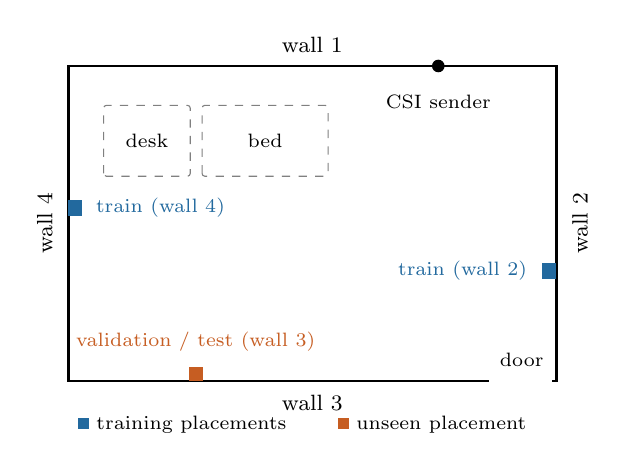
\begin{tikzpicture}[font=\footnotesize]
\draw[line width=1pt] (0,0) rectangle (6.2,4);
\draw[white,line width=1.6pt] (5.35,0) -- (6.15,0);
\draw[line width=1pt] (0,0) -- (5.35,0) (6.15,0) -- (6.2,0);
\node[font=\scriptsize] at (5.76,.27) {door};
\node[anchor=south] at (3.1,4.05) {wall 1};
\node[anchor=north] at (3.1,-.05) {wall 3};
\node[rotate=90] at (-.3,2) {wall 4};
\node[rotate=90] at (6.5,2) {wall 2};
\draw[gray,dashed,rounded corners=1pt] (.45,2.6) rectangle (1.55,3.5);
\node[font=\scriptsize] at (1,3.05) {desk};
\draw[gray,dashed,rounded corners=1pt] (1.7,2.6) rectangle (3.3,3.5);
\node[font=\scriptsize] at (2.5,3.05) {bed};
\fill (4.7,4) circle (.08);
\node[font=\scriptsize,anchor=north] at (4.7,3.75) {CSI sender};
\fill[csiBlue] (0,2.1) rectangle (.18,2.3);
\node[font=\scriptsize,text=csiBlue,anchor=west] at (.23,2.2) {train (wall 4)};
\fill[csiBlue] (6.02,1.3) rectangle (6.2,1.5);
\node[font=\scriptsize,text=csiBlue,anchor=east] at (5.95,1.4) {train (wall 2)};
\fill[radarOrange] (1.53,0) rectangle (1.71,.18);
\node[font=\scriptsize,text=radarOrange,anchor=south] at (1.62,.25) {validation / test (wall 3)};
\node[font=\scriptsize,anchor=west] at (0,-.55) {\textcolor{csiBlue}{\rule{.14cm}{.14cm}} training placements};
\node[font=\scriptsize,anchor=west] at (3.3,-.55) {\textcolor{radarOrange}{\rule{.14cm}{.14cm}} unseen placement};
\end{tikzpicture}}
\par\smallskip
\begin{minipage}[c]{.49\columnwidth}\centering
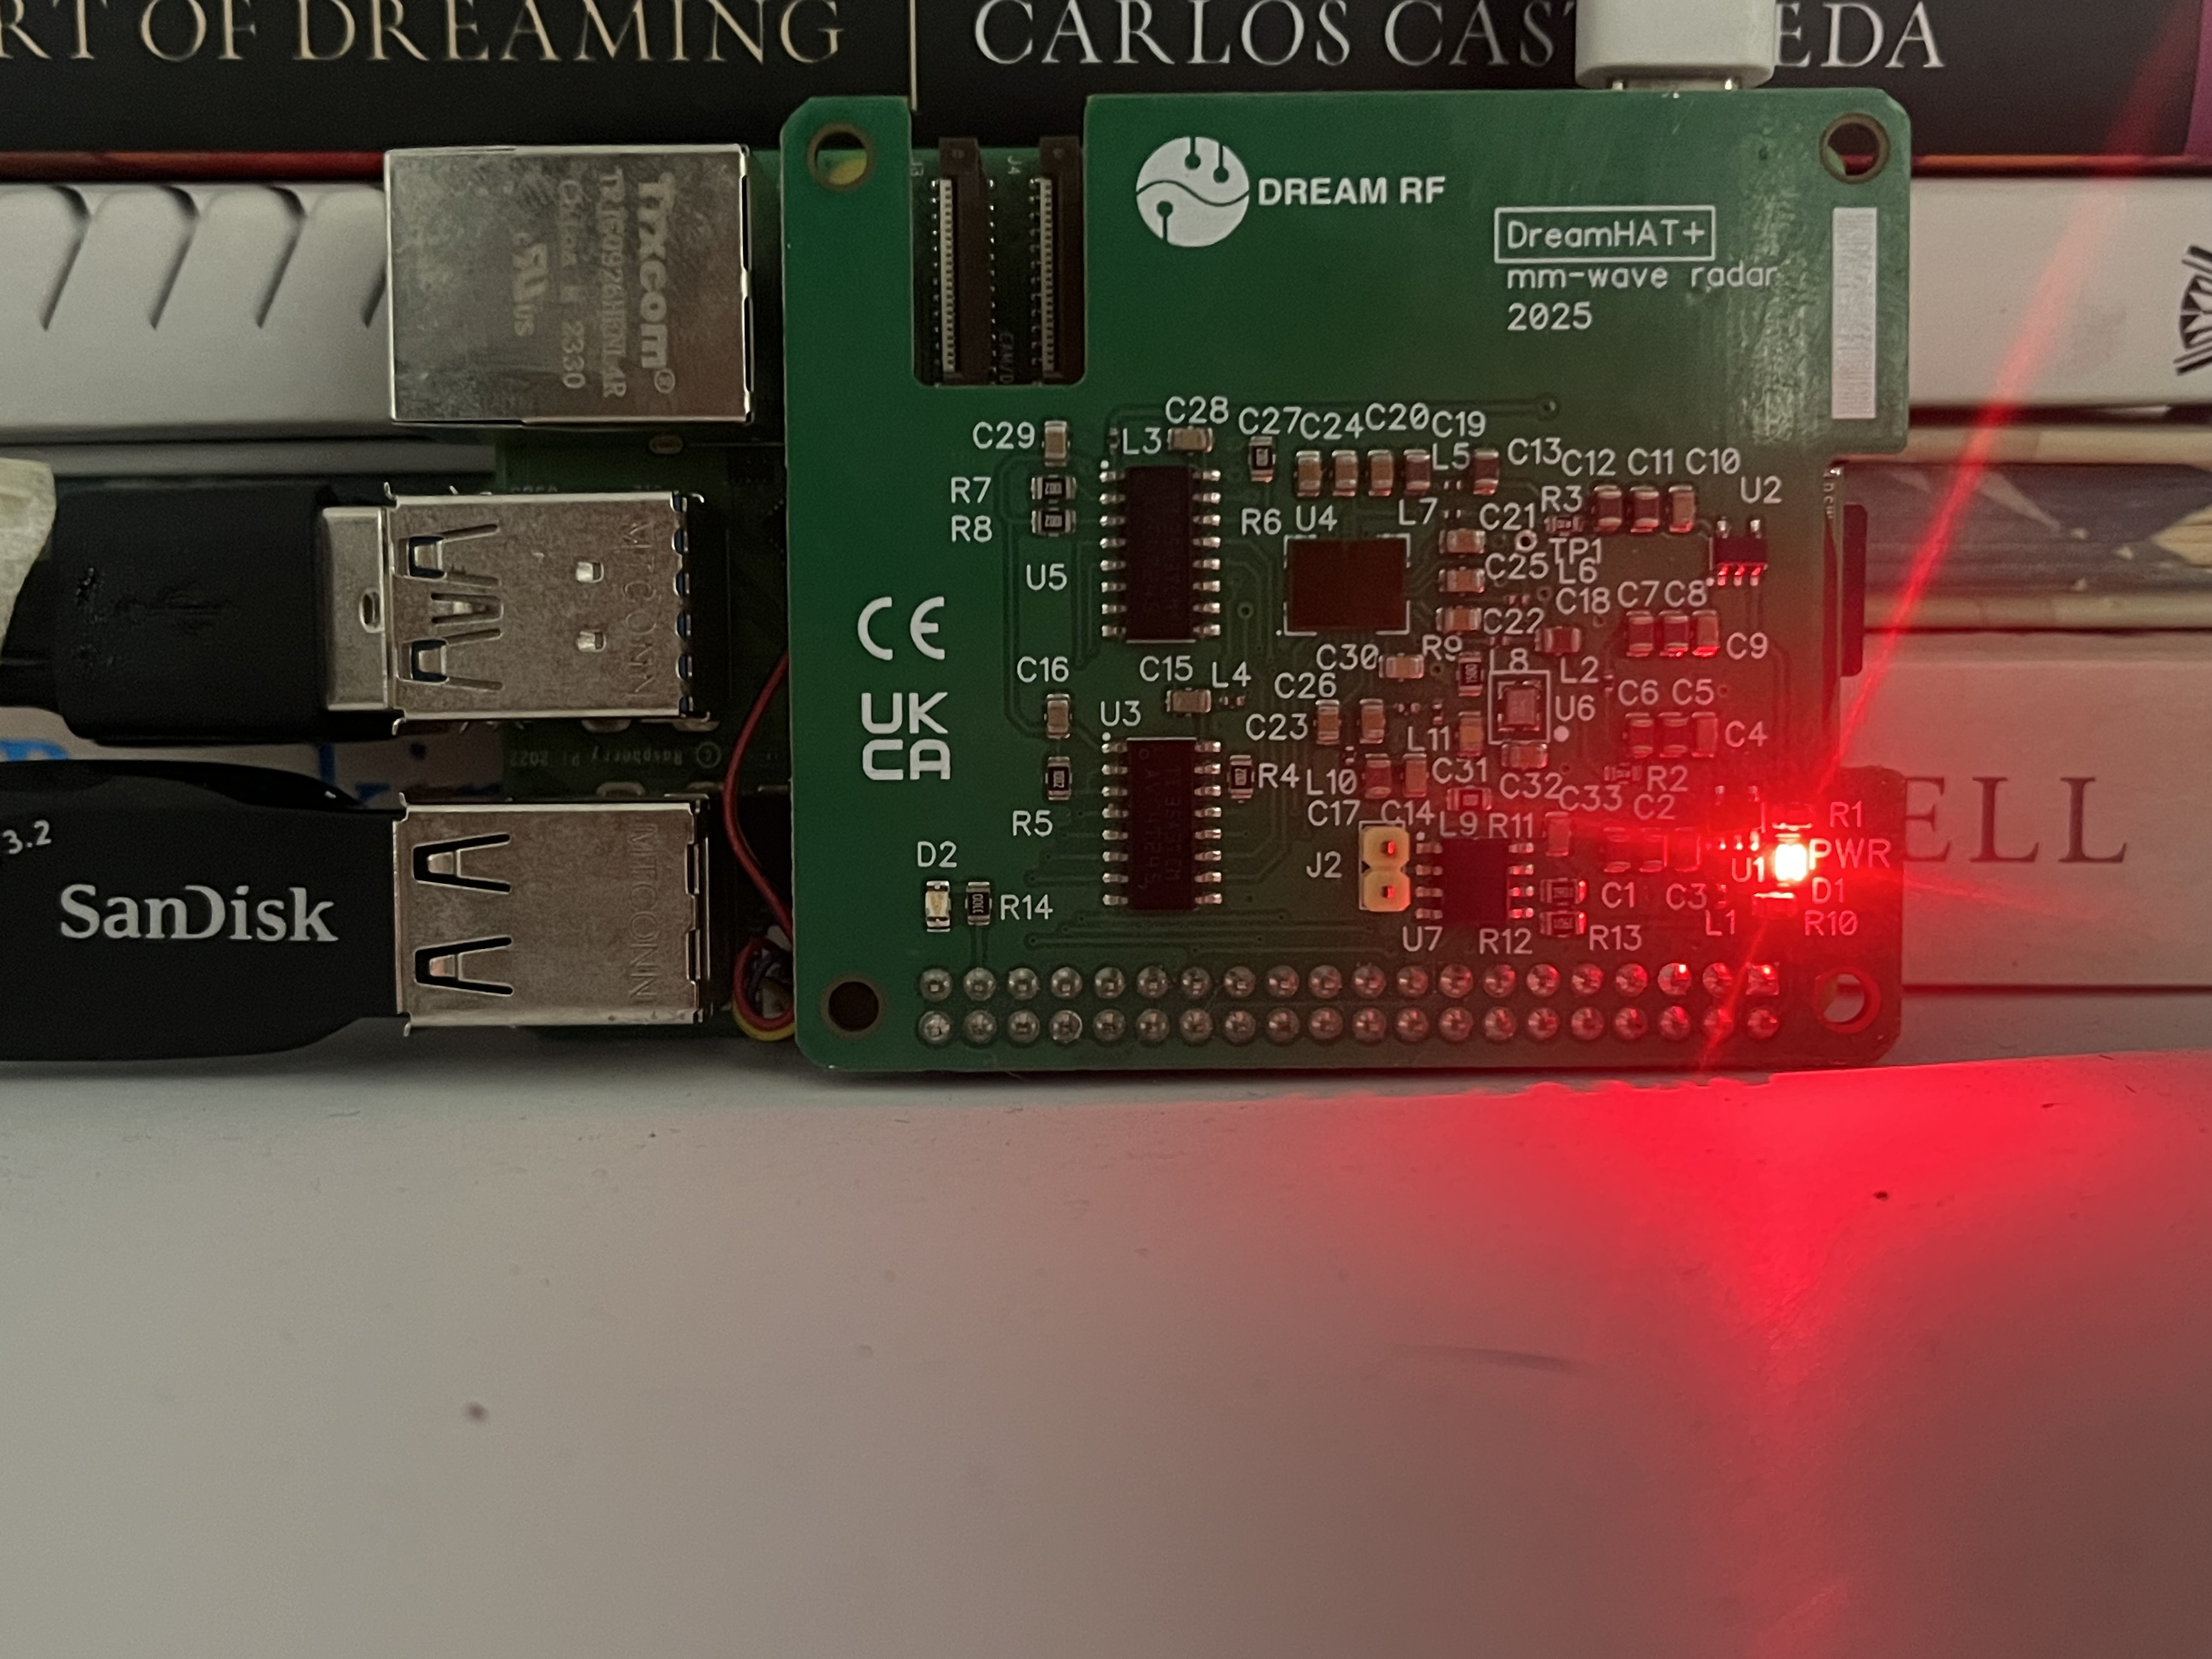
\includegraphics[width=\linewidth,height=2.5cm,keepaspectratio]{IMG_1361.jpeg}\\
{\scriptsize radar: DreamHAT+ on Raspberry Pi}
\end{minipage}\hfill
\begin{minipage}[c]{.49\columnwidth}\centering
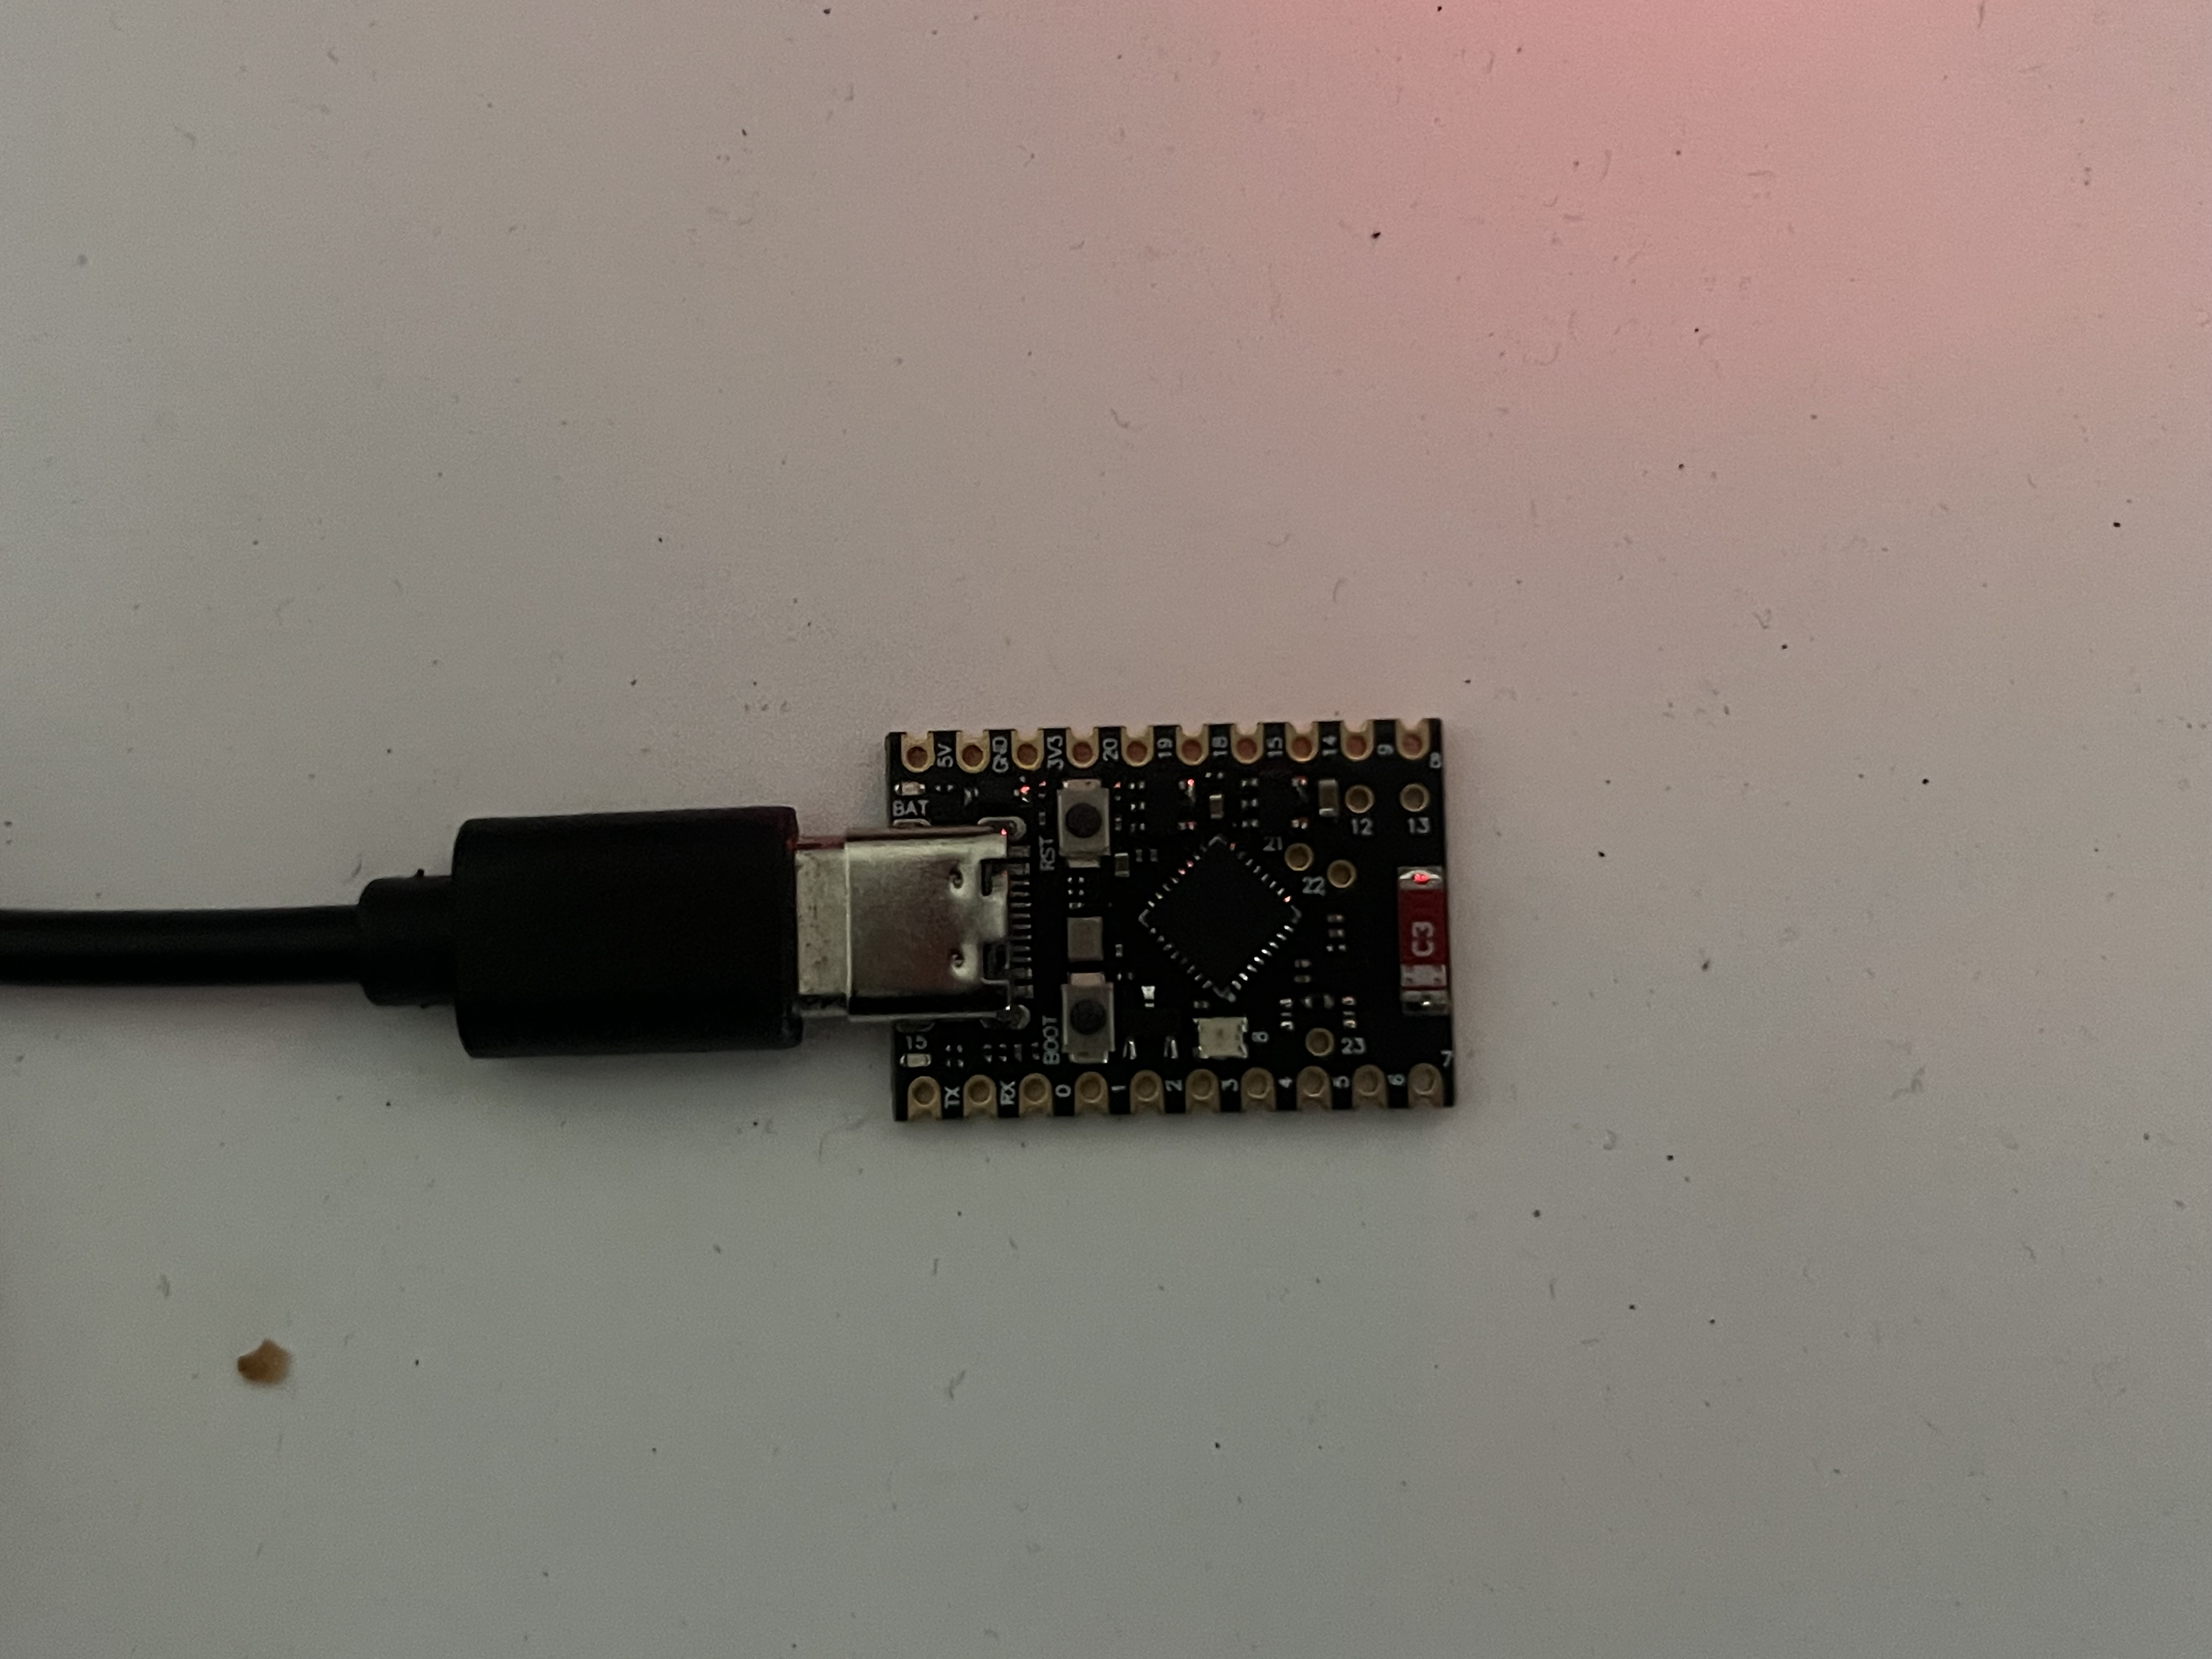
\includegraphics[width=\linewidth,height=2.5cm,keepaspectratio]{IMG_1362.jpeg}\\
{\scriptsize ESP32 board used for CSI}
\end{minipage}
\caption{Room layout, sensor placements, and collection hardware. The co-located FMCW radar and CSI receiver were mounted on wall~4 and wall~2 for training sessions and on wall~3 for validation and test sessions; the CSI sender remained fixed on wall~1. Photographs show the DreamHAT+ mm-wave radar HAT mounted on its Raspberry Pi host (left) and the ESP32 board used for CSI collection (right).}
\label{fig:layout}
\end{figure}

\begin{table}[!b]
\centering\footnotesize
\setlength{\tabcolsep}{3.5pt}
\caption{Sensor configuration. Radar operating band from the BGT60TR13C product brief~\cite{bgt60}; frame structure follows HOOD~\cite{hood}; WiFi settings follow~\cite{wifi}.}
\label{tab:radar}
\begin{tabular}{lcc}\toprule
Configuration & Symbol & Value\\\midrule
\multicolumn{3}{l}{\itshape FMCW radar (BGT60TR13C)}\\
Transmit / receive antennas & $N_{Tx}/N_{Rx}$ & 1 / 3\\
Chirps per frame / samples per chirp & $N_c/N_s$ & 64 / 128\\
Frame period / chirp interval & $T_f/T_{cc}$ & 50\,ms / 391.55\,$\mu$s\\
Start / stop frequency & $f_{\min}/f_{\max}$ & 58 / 63.5\,GHz\\
Bandwidth & $B$ & 5.5\,GHz\\\midrule
\multicolumn{3}{l}{\itshape WiFi CSI (ESP32 sender $\to$ receiver)}\\
Transmit / receive antennas & $N'_{Tx}/N'_{Rx}$ & 1 / 1\\
Channel bandwidth & $B_{\rm wifi}$ & 20\,MHz\\
Reported / retained subcarriers & $K/K'$ & 64 / 52\\
Processed sample grid & $f_s$ & 100\,Hz\\\bottomrule
\end{tabular}
\end{table}

\section{Related Work}
\subsection{WiFi CSI sensing}
CSI exposes per-subcarrier channel gains and has been used for presence, activity, and gesture recognition with commodity hardware. DeMan~\cite{deman} detects both moving and stationary humans by combining motion-induced CSI variation with respiration-induced periodicity, and reports that stationary presence is harder because the signal change is small. SHARP~\cite{sharp} targets environment- and person-independent activity recognition by estimating Doppler traces from CSI phase after sanitization, so that the learned representation depends less on static multipath. LiteHAR~\cite{litehar} replaces deep networks with random convolution kernels and a linear classifier, achieving competitive accuracy with a fraction of the training cost. Our earlier work~\cite{wifi} processes amplitude from ESP32 access points for activity recognition in smart homes and motivates the amplitude-only CSI features used here. These studies generally evaluate on the same device placement used for training or on held-out subjects; placement shift remains a known weakness, and our CSI-only result quantifies it for a fixed-threshold classifier.

\subsection{FMCW radar presence detection}
Millimeter-wave FMCW radar supplies range and Doppler information that does not depend on a separate transmitter link. HOOD~\cite{hood} trains a reconstruction-based detector on the Infineon BGT60TR13C and treats presence detection as an out-of-distribution problem, using range--Doppler inputs and a 60.1--61.1\,GHz ramp in its reported configuration. We use the same radar family but work from logged RD, RA, RE, and XY maps and compute low-dimensional descriptors (energy, temporal variability, peak-to-background) rather than training a reconstruction network, which keeps the models small enough to be summarized in a language-model prompt.

\subsection{Radar--WiFi fusion and explanation}
Chen \emph{et al.}~\cite{fusion} fuse radar and WiFi for cross-scene activity recognition and report that fusion is more stable than either modality alone when the scene changes. We examine the same claim for a binary occupancy task with both early feature concatenation and late probability averaging. For model interpretation, SHAP~\cite{shap} estimates each descriptor's contribution to a prediction; we use it to report which descriptors the frozen models rely on. Supplying model outputs and signal statistics to a large language model for a decision and a textual rationale is a newer practice, and we evaluate whether such rationales add information beyond the supplied model predictions.

\section{System Model}
Let $y_m\in\{0,1\}$ denote empty or occupied in minute $m$. A CSI packet supplies a complex gain $h_i[k]=|h_i[k]|e^{j\phi_i[k]}$ on retained subcarrier $k$; we use the amplitude $|h_i[k]|$. Following HOOD~\cite{hood}, an FMCW chirp is $s(t)=\exp[j2\pi(f_ct+Bt^2/(2T_c))]$ for $0<t<T_c$, with bandwidth $B$ and chirp duration $T_c$; fast-time and chirp-axis FFTs yield range and Doppler. The available radar stream contains logged RD, RA, RE, and XY maps, from which we compute energy, temporal variability, and a peak-to-background proxy rather than HOOD's reconstruction score. The classifier returns $p_m=P(y_m=1\mid x_{1,m},x_{2,m})$. Early fusion concatenates CSI and radar descriptors before classification; late fusion averages separately fitted CSI and radar probabilities. Figure~\ref{fig:layout} shows the room and sensor placements and Table~\ref{tab:radar} lists the sensor configuration. The BGT60TR13C operates in the 58--63.5\,GHz band~\cite{bgt60}; HOOD's reported ramp of 60.1--61.1\,GHz~\cite{hood} lies inside this band. The exact ramp used in each capture is not stored in the available manifests, so Table~\ref{tab:radar} reports the device band.

\section{Data Collection and Processing}
\subsection{Collection protocol}
All data were collected from one subject in the single room shown in Fig.~\ref{fig:layout}. The FMCW radar and the CSI receiver are co-located on one mount; the CSI sender is fixed on wall~1. Training sessions were recorded with the mount on wall~2 and on wall~4. Validation and test sessions were recorded with the mount on wall~3, a placement absent from training, to simulate an unseen domain. Each session runs the multimodal collection (CSI and radar logged together) for a fixed duration under one condition: the subject is present in the room and the session is labeled \emph{occupied}, or the subject leaves and the session is labeled \emph{empty}. Labels are therefore assigned per session, not per frame, and no session contains an occupancy transition.

\subsection{Data sets and preprocessing}
Figure~\ref{fig:sizes} summarizes the data sets. The development collection provides 273 recorded training minutes (187 empty, 86 occupied) and 192 recorded validation minutes (112 empty, 80 occupied). Because occupied is the minority class in both development sets, we synthesize occupied minutes by perturbing each set's own recorded occupied minutes at the descriptor level: Gaussian noise, gain drift, mixup between occupied minutes, and temporal resampling, in rotation. This adds 101 synthetic training and 32 synthetic validation minutes, giving balanced sets of 374 and 224 minutes (4,488 and 2,688 five-second windows). Four multilink test captures (two per class) provide 4,320 windows and 360 minute buckets (180 per class) and are never augmented. Each capture has one label, so minutes are nested within captures. Multilink CSI averages two links per window, unlike single-link development data. An occupied-only calibration session recorded at the training placements is excluded because it cannot inform a two-class rule. Windows without usable CSI are retained as radar-only windows; their CSI descriptors receive training medians. Sleep is occupied where present.

\begin{figure}[!t]
\centering
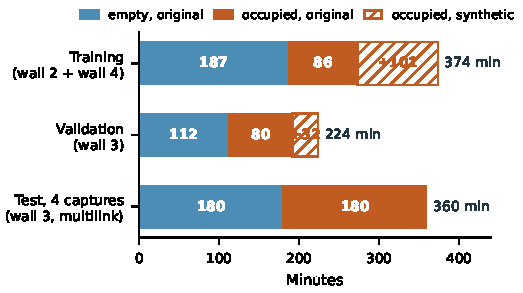
\includegraphics[width=\columnwidth]{data_sizes.pdf}
\caption{Data sizes in minutes per class: recorded (solid) and synthesized occupied minutes added for class balance (hatched). Test captures are never augmented.}
\label{fig:sizes}
\end{figure}

\subsection{Physical and PCA descriptors}
Candidates include CSI amplitude/variance, RD/RA/RE/XY map summaries, and an SNR proxy: $10\log_{10}$ of nonmasked RD peak over median RD power. A development-only screen retains descriptors with consistent training/validation AUC direction and minimum direction-adjusted AUC .55. Figure~\ref{fig:stable} shows the retained RA and RE temporal-variability descriptors, whose direction persists on multilink test. Three peak measures reverse on test; RA and RE means fail the development screen. Each modality also carries compact PCA descriptors: one-second CSI dots (mean/std of the 52 subcarrier amplitudes) and radar dots (flattened mean RD map) are projected onto three-component bases fitted on training recordings only, and each five-second window contributes the mean and standard deviation of its three CSI and three radar coordinates (12 descriptors). Model inputs below always combine the physical and PCA descriptors; Fig.~\ref{fig:pca} shows the training-basis coordinates projected for test seconds.

\begin{figure*}[!t]
\centering
\begin{minipage}[t]{.47\textwidth}
\centering
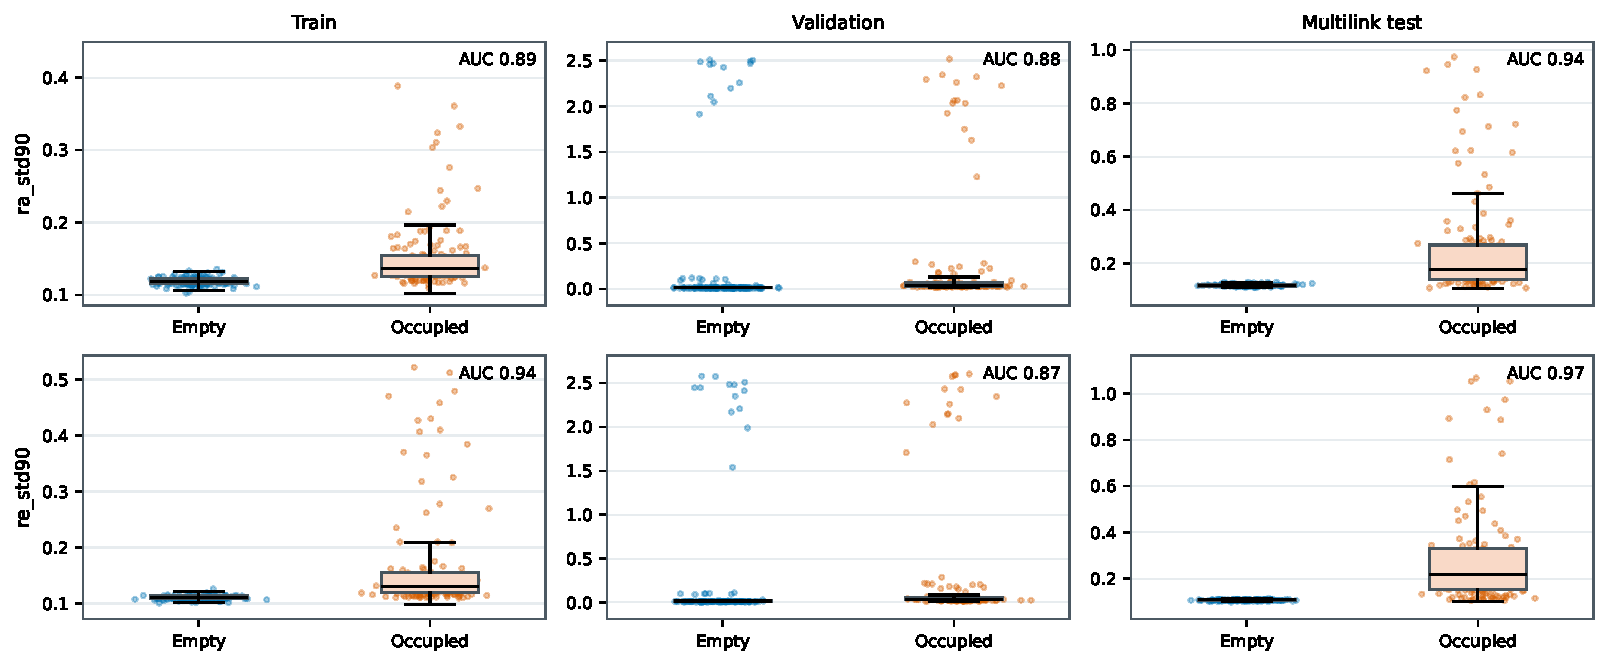
\includegraphics[width=.97\linewidth]{stable_descriptor_box_scatter.pdf}
\caption{RA and RE variability by class in the training, validation, and multilink test sets.}
\label{fig:stable}
\end{minipage}\hfill
\begin{minipage}[t]{.47\textwidth}
\centering
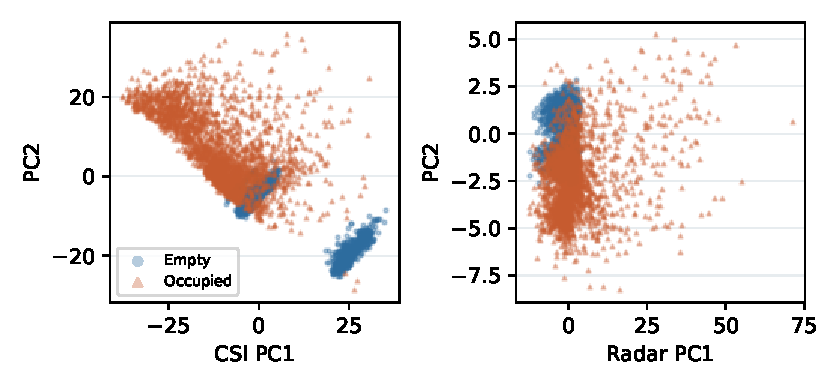
\includegraphics[width=.97\linewidth]{pca_scatter.pdf}
\caption{One-second PC coordinates from training-fitted bases, shown for multilink test seconds; no test fitting.}
\label{fig:pca}
\end{minipage}
\end{figure*}

\section{Predictive Models and Evaluation}
We fit RF, GBM, SVM, and a two-hidden-layer MLP (64/32 units) on CSI, radar, and their early descriptor concatenation, each with five random seeds. Late fusion averages same-family CSI and radar probabilities with fixed equal weights. The balanced training set fits missing-value medians, scalers, and model weights; the balanced validation set fixes each seed's cutoff by balanced accuracy, and mean validation-minute AUC over the five seeds selects each view's model and the conventional (ML) and neural (DL) reference models. All choices precede multilink evaluation. Minute probabilities average twelve five-second outputs; window comparisons use the same minute-fitted cutoff. Test data update no model component.

Classifier vectors contain 14 CSI descriptors (amplitude mean/std/90th percentile; rolling-variance mean/90th percentile/maximum; temporal variance; Doppler fraction; mean/std of three training-basis PCs) and 28 radar descriptors (SNR mean/maximum; mean, 90th percentile, variability, frame delta, and peak for each RD, RA, RE, and XY map; mean/std of three training-basis PCs), giving 42 early-fusion inputs. Each view has training-fitted medians and $z$ scores. Validation fixes the late-fusion GBM and early-fusion MLP reference cutoffs at .662 and .484; Fig.~\ref{fig:workflow} shows their frozen path.

\begin{figure}[H]
\centering
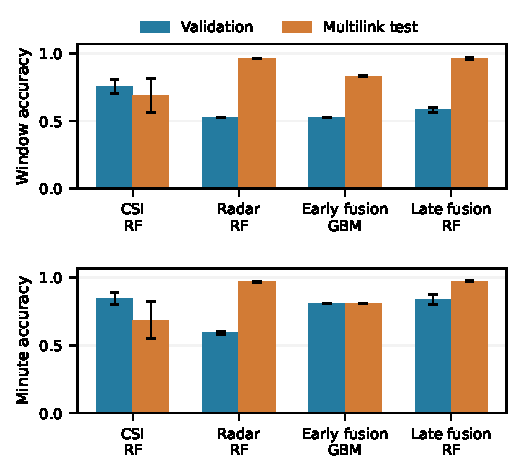
\includegraphics[width=.86\columnwidth]{frozen_comparison.pdf}
\caption{Window and minute accuracy on validation (blue) and multilink test (orange), using validation-fixed models and thresholds.}
\label{fig:pass}
\end{figure}

\section{Language-Model Inference}
Each LLM receives fifteen minute means: CSI amplitude mean/std, rolling variance, and PC1--3 means; radar SNR, RA/RE/XY variability 90th percentiles, RA/RE frame deltas, and PC1--3 means. One request combines a system rule with a JSON user body that adds training-class mean/std, two labeled training-minute examples per class, and each reference's validation-fixed cutoff, balanced accuracy, minute probability, and decision (Fig.~\ref{fig:workflow}). The system rule asks the LLM to respect model agreement and compare cutoff margins with descriptor statistics on disagreement. IDs are shuffled; capture names, labels, and test-batch ranks are excluded. Output probabilities use a fixed .5 decision cutoff. Three runs cover all 224 validation and 360 test minutes with the same frozen prompt.

\begin{figure*}[!t]
\centering
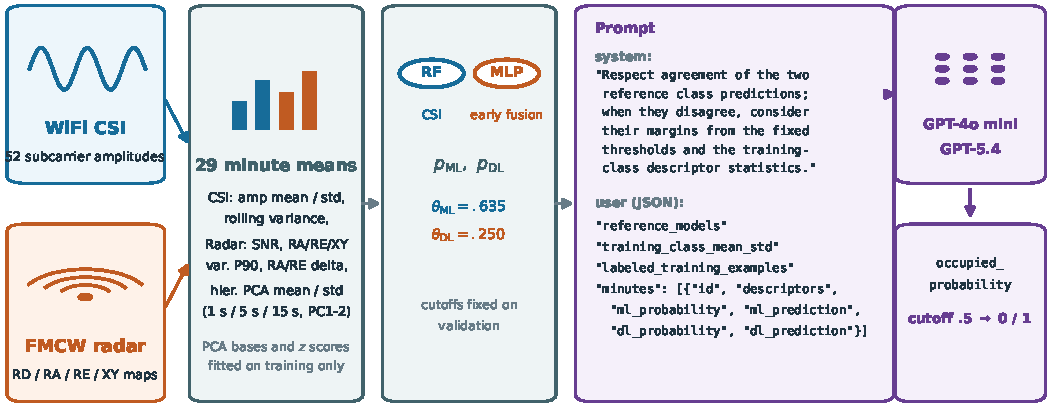
\includegraphics[width=.78\textwidth]{frozen_pipeline.pdf}
\caption{Frozen descriptor-to-LLM path. Fifteen minute-mean descriptors and the late-fusion GBM and early-fusion MLP reference probabilities with their validation-fixed cutoffs enter a single chat request; the card shows the system rule and the JSON user keys. The LLM returns an occupancy probability thresholded at .5.}
\label{fig:workflow}
\end{figure*}

\begin{table*}[!t]
\centering\scriptsize\setlength{\tabcolsep}{2pt}\renewcommand{\arraystretch}{1.0}
\caption{Six multilink minutes (three per class). $A/V$: CSI amplitude/rolling-variance mean; $S$: radar SNR; $R_A/R_E/X$: radar variability. References are late-fusion GBM / early-fusion MLP; LLM reasons are verbatim.}
\label{tab:explain}
\begin{tabular}{@{}lp{.19\textwidth}p{.055\textwidth}p{.325\textwidth}p{.325\textwidth}@{}}
\toprule
ID/actual & Signal summary & Ref. $p$ & GPT-4o mini: prediction, reason & GPT-5.4: prediction, reason \\
\midrule
% Generated by E2/export_explainability_rows_v3.py; reasons are verbatim.
m0133/E & CSI $A/V$: 33.22/0.010\newline Radar $S$: 7.58\newline $R_A/R_E/X$: 0.12/0.11/0.11 & 0.65/\newline 0.00 & \textbf{O (0.65)}. High CSI amplitude and PC1 mean; ML output supports occupancy. & \textbf{E (0.20)}. CSI amplitude/SNR and motion stats look empty-like; radar PCs also near empty. ML barely occupied 0.6485, but DL strongly empty 0.0001. \\
\addlinespace[2pt]
m0286/E & CSI $A/V$: 32.82/0.011\newline Radar $S$: 7.46\newline $R_A/R_E/X$: 0.12/0.11/0.11 & 0.64/\newline 0.00 & \textbf{O (0.64)}. High CSI amplitude and PC1 mean; ML output indicates occupancy. & \textbf{E (0.19)}. CSI motion and SNR are empty-like despite shifted PCA basis; radar PCs remain near empty. ML barely occupied 0.6353, DL strongly empty 0.0002. \\
\addlinespace[2pt]
m0215/E & CSI $A/V$: 23.47/0.008\newline Radar $S$: 7.71\newline $R_A/R_E/X$: 0.12/0.11/0.11 & 0.62/\newline 0.03 & \textbf{E (0.62)}. Low CSI amplitude and PC1 mean; ML output suggests emptiness. & \textbf{E (0.08)}. CSI amplitude, SNR, ra/re spread and deltas match empty; radar PCs modest and non-occupied. Both models predict empty: ML 0.6179, DL 0.0259. \\
\addlinespace[2pt]
m0146/O & CSI $A/V$: 16.27/0.037\newline Radar $S$: 15.49\newline $R_A/R_E/X$: 0.48/0.58/0.36 & 0.70/\newline 1.00 & \textbf{O (0.70)}. High SNR and significant radar PC1 mean; ML output confirms occupancy. & \textbf{O (0.99)}. CSI high SNR, ra/re spreads, deltas, extreme PCs indicate occupancy; radar PC1/PC2 strongly match occupied examples. Both models occupied: ML 0.696, DL 1.0. \\
\addlinespace[2pt]
m0209/O & CSI $A/V$: 16.65/0.018\newline Radar $S$: 7.57\newline $R_A/R_E/X$: 0.16/0.17/0.14 & 0.81/\newline 1.00 & \textbf{O (0.81)}. Strong radar evidence and high ML probability indicate occupancy. & \textbf{O (0.87)}. CSI very low amplitude and strongly shifted PCs support occupancy; radar motion stats are weaker, only mildly occupied-like. Both models occupied: ML 0.8136, DL 1.0. \\
\addlinespace[2pt]
m0147/O & CSI $A/V$: 19.30/0.008\newline Radar $S$: 7.79\newline $R_A/R_E/X$: 0.17/0.23/0.15 & 0.79/\newline 1.00 & \textbf{O (0.79)}. Radar PC1 mean suggests occupancy; ML output supports this. & \textbf{O (0.72)}. CSI lower amplitude, elevated re/xy spread, shifted PCs suggest occupancy; radar PCs conflict, looking atypical/empty-leaning. Both models still occupied: ML 0.7944, DL 0.9979. \\
\bottomrule

\end{tabular}
\end{table*}

\section{Results and Discussion}\label{sec:results}
\begin{table}[!t]
\centering\footnotesize\setlength{\tabcolsep}{3.5pt}
\caption{Five-second models on physical + PCA descriptors, minute evaluation, validation-fixed thresholds; mean $\pm$ sd over five seeds (sd omitted when $<.005$). $^\ast$~view leader by mean validation-minute AUC.}
\label{tab:primary}
\begin{tabular}{llllll}
\toprule
View & Model & Val. AUC & Val. acc. & Test acc. & Test AUC\\
\midrule
\multirow{4}{*}{CSI} & RF & .96$\pm$.00 & .93$\pm$.00 & .89$\pm$.01 & .95$\pm$.01 \\
 & GBM$^\ast$ & .97 & .93 & .94 & .97 \\
 & SVM & .38 & .51 & .54$\pm$.00 & .45 \\
 & MLP & .66$\pm$.21 & .67$\pm$.15 & .53$\pm$.05 & .67$\pm$.05 \\
\midrule
\multirow{4}{*}{Radar} & RF & .61$\pm$.03 & .61$\pm$.02 & .96$\pm$.01 & .99$\pm$.01 \\
 & GBM$^\ast$ & .79 & .74 & .92 & .98 \\
 & SVM & .67 & .61 & .99 & 1.00 \\
 & MLP & .57$\pm$.02 & .59$\pm$.03 & .50 & .74$\pm$.06 \\
\midrule
\multirow{4}{*}{Early fusion} & RF & .67$\pm$.18 & .67$\pm$.10 & .95$\pm$.00 & .99$\pm$.00 \\
 & GBM$^\ast$ & .97 & .93 & .94 & .99 \\
 & SVM & .60$\pm$.00 & .60 & .49 & .55$\pm$.00 \\
 & MLP & .76$\pm$.27 & .77$\pm$.18 & .56$\pm$.09 & .81$\pm$.05 \\
\midrule
\multirow{4}{*}{Late fusion} & RF & .97$\pm$.00 & .93$\pm$.01 & .98$\pm$.01 & 1.00 \\
 & GBM$^\ast$ & .98 & .93 & .99 & 1.00 \\
 & SVM & .45$\pm$.00 & .52 & .99$\pm$.00 & 1.00 \\
 & MLP & .68$\pm$.18 & .68$\pm$.15 & .56$\pm$.07 & .65$\pm$.07 \\
\bottomrule
\end{tabular}
\end{table}

\begin{figure}[!t]
\centering
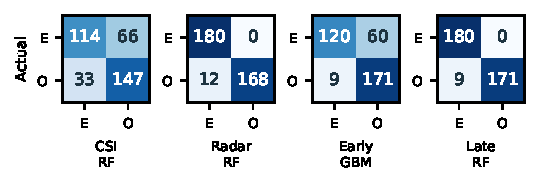
\includegraphics[width=.9\columnwidth]{primary_cm.pdf}
\caption{Test confusion matrices for Table~\ref{tab:primary}'s view leaders over 360 minutes. E/O: empty/occupied; rows are actual, columns predicted.}
\label{fig:primarycm}
\end{figure}

\subsection{CSI-only results}
The CSI GBM leads its view on validation (AUC .97, accuracy .93) and retains .94 test minute accuracy (window .88), markedly better than an earlier physical-only CSI model. Its confusion matrix misclassifies 10 empty and 12 occupied minutes (Table~\ref{tab:primary}, Fig.~\ref{fig:primarycm}). The neural MLP is again unstable across seeds (test $.53\pm.05$): CSI transfers in ranking but not reliably in calibration.

\subsection{Radar-only results}
The validation-selected radar GBM reaches .741 validation and .922 test minute accuracy; the corresponding window accuracies are .572 and .915 with the same minute-fitted threshold. A radar SVM scores .992 on test, but its validation AUC (.67) is below GBM's (.79), so the frozen rule cannot pick it. The test evaluates two captures per class whose labels do not change within a capture.

\subsection{Sensor fusion: early features}
Early fusion concatenates the 42 CSI and radar descriptors before fitting. The GBM leader matches the CSI view on validation (.93) and test (.94), with the best test window accuracy (.956) of the four views. RF early fusion scores $.95\pm.00$ test, close to its fusion counterpart.

\subsection{Decision fusion: late probabilities}
Late fusion averages same-family CSI and radar probabilities with weight $1/2$ fixed before evaluation. The GBM pair reaches .933 validation and .986 test minute accuracy (window .943, test AUC 1.00); the RF pair follows at $.98\pm.01$ test. Late fusion is again the strongest selectable view. The test includes two independent captures per class, with correlated minutes within each capture.

\subsection{Descriptor importance}
Table~\ref{tab:shap} reports interventional Shapley estimates for the ML reference (late-fusion GBM), the DL reference (early-fusion MLP), and the early-fusion GBM. Each of 24 random descriptor orders starts from a random training window; 24 validation windows (12 per class) are explained. For late fusion the largest contributions are CSI PC3 mean (.121), RA peak (.108), and CSI amplitude P90 (.107). The DL reference concentrates on RE peak (.271), RA peak (.243), and CSI amplitude P90 (.168); the early GBM on RA peak (.260), CSI amplitude P90 (.160), and RE variability (.128). PCA coordinates rank among the top contributors for the ML reference, while radar PCs contribute little. These values describe model reliance, not causal sensor importance~\cite{shap}; neither SHAP sampling nor model choice uses multilink labels.

\begin{table}[!t]
\centering\scriptsize\setlength{\tabcolsep}{5pt}
\caption{Mean absolute interventional Shapley contribution to occupied probability for the ML reference (late-fusion GBM), the DL reference (early-fusion MLP), and the early-fusion GBM (Early); 24 validation windows, training-window background.}
\label{tab:shap}
\begin{tabular}{@{}llll@{}}
\toprule
Descriptor & ML & DL & Early\\
\midrule
CSI amplitude mean & .049 & .208 & .095 & RA energy mean & -- & .432 & .001 \\
CSI amplitude std & .074 & .007 & .020 & RA energy P90 & -- & .413 & .000 \\
CSI amplitude P90 & .157 & .126 & .219 & RA variability P90 & -- & .023 & .001 \\
CSI rolling-var. mean & .011 & .004 & .004 & RA frame delta & -- & .091 & .000 \\
CSI rolling-var. P90 & .007 & .004 & .004 & RA peak/background & -- & .088 & .006 \\
CSI rolling-var. max & .003 & .006 & .005 & RE energy mean & -- & .176 & .000 \\
CSI total variation & .026 & .007 & .014 & RE energy P90 & -- & .128 & .003 \\
CSI Doppler fraction & .013 & .005 & .008 & RE variability P90 & -- & .032 & .132 \\
CSI 1 s PC1 mean & .024 & .095 & .032 & RE frame delta & -- & .071 & .081 \\
CSI 1 s PC2 mean & .005 & .081 & .014 & RE peak/background & -- & .128 & .000 \\
CSI 1 s PC1 std & .015 & .007 & .008 & XY energy mean & -- & .042 & .000 \\
CSI 1 s PC2 std & .009 & .015 & .003 & XY energy P90 & -- & .045 & .000 \\
CSI 5 s PC1 mean & .024 & .026 & .006 & XY variability P90 & -- & .080 & .011 \\
CSI 5 s PC2 mean & .006 & .003 & .007 & XY frame delta & -- & .096 & .000 \\
CSI 5 s PC1 std & .015 & .005 & .011 & XY peak/background & -- & .034 & .002 \\
CSI 5 s PC2 std & .015 & .011 & .002 & Radar 1 s PC1 mean & -- & .004 & .000 \\
CSI 15 s PC1 & .011 & .080 & .013 & Radar 1 s PC2 mean & -- & .048 & .000 \\
CSI 15 s PC2 & .007 & .009 & .004 & Radar 1 s PC1 std & -- & .003 & .000 \\
Radar SNR mean & -- & .003 & .000 & Radar 1 s PC2 std & -- & .006 & .000 \\
Radar SNR max & -- & .002 & .000 & Radar 5 s PC1 mean & -- & .032 & .000 \\
RD energy mean & -- & .002 & .000 & Radar 5 s PC2 mean & -- & .009 & .000 \\
RD energy P90 & -- & .009 & .000 & Radar 5 s PC1 std & -- & .035 & .000 \\
RD variability P90 & -- & .002 & .000 & Radar 5 s PC2 std & -- & .002 & .000 \\
RD frame delta & -- & .011 & .000 & Radar 15 s PC1 & -- & .030 & .000 \\
RD peak/background & -- & .047 & .001 & Radar 15 s PC2 & -- & .013 & .000 \\
\bottomrule
\end{tabular}
\end{table}

\subsection{Language-model evaluation}
GPT-4o mini scores $68.8\pm0.4$\% on validation and $59.7\pm1.2$\% on multilink test; GPT-5.4 scores $96.0\pm0.0$\% and $95.7\pm0.3$\%, respectively (mean $\pm$ sample standard deviation over three runs). For run~1 on all 360 test minutes, the confusion counts (true empty, false occupied, false empty, true occupied) are $(38,142,0,180)$ for GPT-4o mini, $(168,12,4,176)$ for GPT-5.4, $(180,0,5,175)$ for late-fusion GBM, and $(0,180,4,176)$ for the early-fusion MLP reference. GPT-4o mini predicts occupied for almost every minute, tracking the DL reference, which itself fails on test (.56 accuracy, all empty minutes missed); GPT-5.4 instead discounts that reference and approaches, but does not reach, the fused GBM's .986. Run-to-run spread reuses the same minutes, so it is not an independent-sample interval.

\subsection{LLM explanation check}
For a separate qualitative check, we selected three empty and three occupied test minutes by fixed-seed sampling within the four captures, without considering model outcomes. Both LLMs received the same fifteen descriptors and frozen reference outputs as above, with a request for a short reason; this prompt differs and is excluded from the accuracy estimate. Table~\ref{tab:explain} reports their complete concise replies. GPT-4o mini follows the DL reference and calls every sample occupied, including three empty ones. GPT-5.4 explicitly notes the DL reference's out-of-distribution behaviour on the empty minutes and resolves all six correctly from the physical descriptors. These are model-generated rationales, not causal explanations of raw signals.

\section{Limitations}
Labels are constant within each capture, so adjacent minutes are correlated, occupancy transitions are not measured, and capture replication is two per class. The unseen domain is a placement change for one subject in one room, the per-capture radar ramp is not logged (Table~\ref{tab:radar} reports the device band), and descriptor-level synthetic minutes add no information beyond the recorded ones. The LLM prompt asks for agreement with two supplied decisions, and a plausible rationale is not an independent explanation of the measurement.

\section{Conclusion}
Physical and training-fitted PCA descriptors together drive the five-second models, and descriptor-level augmentation balances the training and validation sets. Under validation-fixed models and thresholds, the selected GBM views reach .939 CSI, .922 radar, .942 early-fusion, and .986 late-fusion minute accuracy on the unseen test placement. GPT-4o mini reaches .597 test accuracy by tracking a neural reference that fails there; GPT-5.4 reaches .957. Neither exceeds the late-fusion GBM, and generated rationales can echo a failing reference. The remaining gaps are within-session occupancy transitions, additional subjects and rooms, and logged per-capture radar settings.

\begin{thebibliography}{8}
\bibitem{wifi} G. Gad, M. Fouda, and Z. M. Fadlullah, ``WiFi sensing-based human activity recognition for smart home applications using commodity access points,'' manuscript, 2026.
\bibitem{bgt60} Infineon Technologies, ``BGT60TR13C 60\,GHz radar sensor: Product brief,'' 2025. [Online]. Available: \url{https://cdn.shopify.com/s/files/1/0174/1800/files/Product_Brief.pdf}
\bibitem{hood} S. M. Kahya, M. S. Yavuz, and E. Steinbach, ``HOOD: Real-time human presence and out-of-distribution detection using FMCW radar,'' arXiv:2308.02396v2, Mar. 2024.
\bibitem{deman} C. Wu \emph{et al.}, ``Non-invasive detection of moving and stationary human with WiFi,'' \emph{IEEE J. Sel. Areas Commun.}, vol. 33, no. 11, pp. 2329--2342, 2015.
\bibitem{sharp} F. Meneghello \emph{et al.}, ``SHARP: Environment and person independent activity recognition with commodity IEEE 802.11 access points,'' \emph{IEEE Trans. Mobile Comput.}, 2023.
\bibitem{litehar} H. Salehinejad and S. Valaee, ``LiteHAR: Lightweight human activity recognition from WiFi signals with random convolution kernels,'' in \emph{Proc. ICASSP}, 2022.
\bibitem{fusion} Z. Chen, Y. Sun, and L. Qu, ``Research on cross-scene human activity recognition based on radar and Wi-Fi multimodal fusion,'' \emph{Electronics}, vol. 14, no. 8, p. 1518, 2025.
\bibitem{shap} S. M. Lundberg and S.-I. Lee, ``A unified approach to interpreting model predictions,'' in \emph{Advances in Neural Information Processing Systems}, 2017.
\end{thebibliography}
\end{document}

